%%%%%%%%%%%%%%%%%%%%%%%%%%%%%%%%%%%%%%%%%%%%%%%%%%%%%%%%%%%%%%%%
%
%  Template for creating scribe notes for cs229t. borrowed from Rob Schapire 
%
%  Fill in your name, lecture number, lecture date and body
%  of scribe notes as indicated below.
%
%%%%%%%%%%%%%%%%%%%%%%%%%%%%%%%%%%%%%%%%%%%%%%%%%%%%%%%%%%%%%%%%


\documentclass[11pt]{article}

\setlength{\topmargin}{0pt}
\setlength{\textheight}{9in}
\setlength{\headheight}{0pt}
\setlength{\headsep}{0pt}
\setlength{\oddsidemargin}{0.25in}
\setlength{\textwidth}{6in}

\newcommand{\draftnotice}{\vbox to 0.25in{\noindent
   \raisebox{0.6in}[0in][0in]{\makebox[\textwidth][r]{\it
    DRAFT --- a final version will be posted shortly}}}
   \vspace{-.25in}\vspace{-\baselineskip}
}
\makeatletter
\newcommand\xleftrightarrow[2][]{%
  \ext@arrow 9999{\longleftrightarrowfill@}{#1}{#2}}
\newcommand\longleftrightarrowfill@{%
  \arrowfill@\leftarrow\relbar\rightarrow}
\makeatother

\newcommand{\overbar}[1]{\mkern 1.5mu\overline{\mkern-1.5mu#1\mkern-1.5mu}\mkern 1.5mu}

\pagestyle{plain}
\usepackage{amsthm}
\usepackage{amsmath}
\usepackage{amssymb}
\usepackage{bm}
\usepackage{bbm}
\usepackage{dsfont}
\usepackage{graphicx}
\usepackage{subfigure}
\usepackage{float}

\usepackage{tcolorbox}
\newtheorem{theorem}{Theorem}
\newtheorem{lemma}{Lemma}
\newtheorem{claim}{Claim}
\theoremstyle{definition}
\newtheorem{definition}{Definition}

\theoremstyle{remark}
\newtheorem{remark}[theorem]{Remark}
\DeclareMathOperator{\E}{\mathbb{E}}
\begin{document}

\thispagestyle{empty}

% \draftnotice

\begin{center}
\bf\large CS229T/STATS231: Statistical Learning Theory
\end{center}

\noindent
Lecturer: Tengyu Ma   %%% FILL IN LECTURER (if not RS)
\hfill
Lecture \#9               %%% FILL IN LECTURE NUMBER HERE
\\
Scribe: Bo Liu, Zhaozhuo Xu                 %%% FILL IN YOUR NAME 
\hfill
October 22, 2018           %%% FILL IN LECTURE DATE HERE

\noindent
\rule{\textwidth}{1pt}

\medskip

%%%%%%%%%%%%%%%%%%%%%%%%%%%%%%%%%%%%%%%%%%%%%%%%%%%%%%%%%%%%%%%%
%% BODY OF SCRIBE NOTES GOES HERE
%%%%%%%%%%%%%%%%%%%%%%%%%%%%%%%%%%%%%%%%%%%%%%%%%%%%%%%%%%%%%%%%

\section{Review and Overview}
This lecture mainly covers three topics:
\begin{itemize}
	\item Wrap up the proof for the margin based generalization error of the two-layer neural network from the last lecture.
	\item For finite hypothesis, introduce the shattering coefficient (the growth function) that measures the richness of the hypothesis set and the Massart's lemma that relates the Rademacher Complexity to the growth function. Then introduce the concept of VC dimension and explains how it relates to the above.
	\item Lastly, recall the covering technique and use it to deal with infinite hypothesis.
\end{itemize}  

\section{Margin Theory of Neural Network (continued)}
Recall from the last lecture, we define the $\lambda$-regularized exponential loss as:
\[
L_{\lambda}(\theta)=\frac{1}{n}\sum \limits_{i=1}^{n}\exp(-y_if(x_i))+\lambda||\theta||_{2}^{2}
\]
\begin{tcolorbox}[standard jigsaw, opacityback=0]
\textbf{Digression}: here we briefly show why we can replace the logistic loss with the exponential loss for easier derivation.\\\\
Recall that
\[\text{logistic loss} = \sum \limits_{i=1}^n \log \bigg(1 +\exp{ \big(-y_i f_\theta(x_i)\big)}  \bigg)\]
If the margin $y_i f_\theta(x_i)$ is large, it means $t = \exp{ \big(-y_i f_\theta(x_i)\big)}$ is small. Since 
\[\log{\big(1+t\big)} \approx t \quad \text{as} \quad t \to 0 \]
the exponential loss is very close to the logistic loss while being easier to deal with.
\end{tcolorbox}
Then we continue the proof from last lecture\cite{wei2018margin}. Recall the following notations:
\begin{flalign*}
\text{the normalized margin} : \quad \gamma_\theta &\triangleq \min_i y_i f_{\bar{\theta}}(x_i) \qquad \text{where}\quad \bar{\theta} = \frac{\theta}{||\theta||} \\
\text{the max normalized margin}:\quad \gamma^* &= \max_{||\theta||\leq 1} \gamma_{\theta} \\
\text{parameters that achieve the maximum}:\quad \theta^* &\in \arg\max_{||\theta||\leq 1} \gamma_{\theta} \\
\end{flalign*}

\begin{definition}[Positive homogeneity]
    A function $f_\theta$ is positive homogeneous if
    \[\exists c > 0 \quad \text{such that} \quad \forall a > 0\,\,\,\text{and}\,\,\,\forall x \quad f_{a\theta}(x) = a^c f_\theta(x)\]
    Notice that feed forward neural network with ReLU activation is positive homogeneous.
\end{definition}

\begin{theorem}\label{th1}
Let $\gamma_\lambda=\min \limits_{i}y_if_{\overbar{\theta_\lambda}} (x_i)$ be the normalized margin of the global optimizer of $L_\lambda$. Assume $\gamma^*>0$, then as $\lambda \to 0$, $\gamma_\lambda \to \gamma^* $
\end{theorem}

\begin{proof} (Assume $c = 2$ for simplicity)\\\\
Let $S=||\theta_{\lambda}||_2$, according to the definition of $\theta^*$, $||\theta^*||_2=1$ because otherwise we can always scale $\theta^*$ to norm $1$ with a larger normalized margin. Then we have:
\[
||S\theta^*||_2=||\theta_\lambda||_2=S
\]
As  $\theta_\lambda$ is the global optimizer of $L_\lambda$,
\begin{flalign*}
L_\lambda(\theta_\lambda) &\leq L_\lambda(S\theta^*) \\
\frac{1}{n}\sum \limits_{i=1}\exp\bigg(-y_if_{\theta_{\lambda}}(x_i)\bigg)+\lambda||\theta_\lambda||_{2}^{2} &\leq \frac{1}{n}\sum \limits_{i=1}\exp\bigg(-y_if_{S\theta^*}(x_i)\bigg) +\lambda||S\theta^*||_{2}^{2}\\
\overbrace{\frac{1}{n}\sum \limits_{i=1}^n \exp\bigg(-y_if_{\theta_{\lambda}}(x_i)\bigg)}^{(1)} &\leq \overbrace{\frac{1}{n}\sum \limits_{i=1}^n \exp\bigg(-y_if_{S\theta^*}(x_i)\bigg)}^{(2)}
\end{flalign*}
As in the two layer neural network case, $f_{S\theta^*}(x_i)=S^2 f_{\theta^*}(x_i)$ by positive homogeneity when $c=2$. Combining that with the definition of normalized margin over $\gamma^*$, we have  
\begin{flalign*}
(2) &= \frac{1}{n} \sum\limits_{i=1}^n \exp\bigg(-y_i S^2 f_{\theta^*}(x_i)\bigg) \quad\,\,\,\,\, \text{(by homogeneity)} \\
&\leq \frac{1}{n}\sum \limits_{i=1}^n \exp\left(-S^2\gamma^*\right) \qquad \qquad \quad \,\,\, (\text{since } y_i f_{\theta^*}(x_i) \geq \gamma^*)\\
&=\exp\left(-S^2\gamma^*\right)\\
(1) &= \frac{1}{n} \sum\limits_{i=1}^n \exp\bigg(-y_i S^2 f_{\overbar{\theta_\lambda}}(x_i)\bigg) \qquad (\text{define } \overbar{\theta_\lambda} = \frac{\theta_\lambda}{S}) \\
&\geq \frac{1}{n} \exp\left(-S^2\gamma_\lambda\right) \qquad \qquad \qquad \quad\, (\text{since } \exists i, \,\,\, y_i f_{\overbar{\theta_\lambda}}(x_i) = \gamma_{\lambda})
\end{flalign*}
Combined with the fact that $(1) \leq (2)$ from above, we have
\[
\frac{1}{n} \exp\left(-S^2\gamma_\lambda\right) \leq \exp\left(-S^2\gamma^*\right)
\]
which implies
\[
\gamma^*-\gamma_\lambda\leq \frac{\log(n)}{S^2}
\]
Notice that while $n$ is fixed, we can change $S$.

\begin{claim}
As $\lambda\to 0$, $S\to \infty$.
\end{claim}
\begin{proof}
First we note that as $\lambda \rightarrow 0$, $L_{\lambda}(\theta_{\lambda}) \rightarrow 0$. This is because $$L_{\lambda}(\theta_{\lambda}) \le L_{\lambda}(B\theta^\star) \le \exp(-B^2 \gamma^\star) + \lambda B^2$$ and so we can choose $B$ sufficiently large and $\lambda$ sufficiently small to make the upper bound on $L_{\lambda}(\theta_{\lambda})$ arbitrarily small. 

Also note that from the same reasoning as before, $$L_{\lambda}(\theta_{\lambda}) \ge \frac{1}{n} \exp(-S^2 \gamma_{\lambda}) \ge \frac{1}{n} \exp(-S^2 \gamma^\star)$$ where the last inequality follows because $\gamma_{\lambda} \le \gamma^\star$. Thus if $S$ remains bounded as $\lambda \rightarrow 0$, $L_{\lambda}(\theta_{\lambda})$ will be lower bounded by some constant, a contradiction. 
\end{proof}
With this claim,
\[
\lim_{\lambda\to 0} \gamma^*-\gamma_\lambda\leq 0 \Longleftrightarrow \lim_{\lambda\to 0} \gamma^* \leq \gamma_\lambda
\]
Meanwhile, by definition,
\[
\forall \lambda > 0, \,\, \gamma^* \geq \gamma_\lambda
\]
Combine above two equations together, we reach the desired conclusion
\[\lim_{\lambda\to 0} \gamma^*=\gamma_\lambda\]
\end{proof}
\textbf{Recap:} the above shows that minimizing logistic loss with weak regularization will result in a max margin solution. Good margin leads to better generalization by Rademacher Complexity.

% Theorem slightly more general version

% Assume ${f_{\theta}}$ is a set of positive homogeneous functions, then we have
% \[
% \exists c>0 \quad such \ that \quad\forall a>0, \quad\forall x,\quad f_{a\theta}(x)=a^cf_{\theta}(x)  
% \]
% feed forward NN with ReLU is a positive homogeneous function

% Let $\theta_{\lambda}$ be the global minimizer of regulized loss $L_{\lambda}$, we have
% \[
% \gamma_{\lambda}=\gamma_{\theta_{\lambda}}\quad \gamma_{\lambda}\to \gamma^* \quad as\ \lambda\to 0
% \]
% $\lambda\to 0$, ther is no effect, but $\lambda$ has to be small.

% Proof of $c=2$ for simplicity, which means a two layer network.

\section{Growth Function and VC Dimension} 
Consider the binary classification setup with binary loss function:
\[
\mathcal{H} = \{ \, x \longmapsto h (x) \in \{\pm 1\}\,\}
\]
\[
\mathcal{F}=\{(x,y)\longmapsto l((x,y),h): h\in\mathcal{H}\} \quad \text{where}\quad l((x,y),h) \triangleq \mathds{1}(y \neq h(x))
\]
Here $\mathcal{H}$ is the hypothesis set with binary outcomes and $\mathcal{F}$ is the family of loss functions associated to $\mathcal{H}$. Let 
\[
Q_{z_1,...,z_n}=\{\big(f(z_1),...,f(z_n)\big) \in \mathbb{R}^n : f\in \mathcal{F}\}
\]
be all possible outputs from $\mathcal{F}$ on the input sequence $z_1, z_2, \dots, z_n$, where $z_i = (x_i, y_i)$. We can re-define the Rademacher Complexity as
\[
R_s(\mathcal{F}) = \frac{1}{n}\E_{\sigma_i \in \{\pm 1\}^n}
\bigg[\sup \limits_{\bm{q}\in Q} \langle \bm{\sigma}, \bm{q} \rangle \bigg]
\]
since
\[\bm{q} = \begin{bmatrix}
f(z_1) \\ f(z_2) \\ \vdots \\ f(z_n)
\end{bmatrix} \qquad \text{for some } f \in \mathcal{F}
\]
\\
We will then introduce the growth function and use the Massart's lemma to show its relationship to the Rademacher Complexity.\\
\begin{definition}[Growth Function]
The growth function, a.k.a the shattering coefficient is
\[ S(\mathcal{F}, n) \triangleq \max\limits_{z_1, \dots, z_n} \bigg| Q_{z_1, \dots, z_n}\bigg| \qquad \text{with $Q$ defined as in above} \]
\end{definition}
\begin{lemma}[Equivalent Version of Massart's Lemma]
Suppose $Q \subseteq [-1,1]^n$ is finite
\[
R_s(\mathcal{F}) = \frac{1}{n}\E_{\sigma_i \in \{\pm 1\}^n}
\bigg[\sup \limits_{\bm{q}\in Q} \langle \bm{\sigma}, \bm{q} \rangle \bigg] \leq \sqrt{\frac{2\log |Q|}{n}}
\]
\end{lemma}
Therefore, combine Massart's lemma with the growth function, we have
\begin{equation}
R_s(\mathcal{F}) \leq \sqrt{\frac{2\log{|Q|}}{n}} \Longrightarrow R_n(\mathcal{F}) \leq \sqrt{\frac{2\log {S(\mathcal{F}, n)} }{n}}
\end{equation}
because
\[R_n(\mathcal{F}) = \E_{z}[R_s(\mathcal{F})] \leq \max_{z} R_s(\mathcal{F}) \leq \max_{z}\sqrt{\frac{2\log{|Q|}}{n}} \leq \sqrt{\frac{2\log {S(\mathcal{F}, n)} }{n}} \]
This implies that the growth function can be used to bound the Rademacher Complexity.
\\\\\\
Furthermore, for binary loss, the shattering coefficient of loss is the same as the shattering coefficient of the hypothesis class. Because there exists a bijection between the loss and the hypothesis:
\begin{flalign*}
\bigg(l((x_1, y_1), h),\, \dots,\, l((x_n, y_n), h)\bigg) &= \bigg(\mathds{1}(y_1 \neq h(x_1)),\, \dots, \,\mathds{1}(y_n \neq h(x_n))\bigg) \\
&\xleftrightarrow{\text{bijection}} \bigg(h(x_1),\, \dots, \,h(x_n) \bigg)
\end{flalign*}
As a sanity check, it is easy to observe that
\[\bigg| l((x_1, y_1), h),\, \dots,\, l((x_n, y_n), h) : h \in \mathcal{H} \bigg| = \bigg| h(x_1),\, \dots, \,h(x_n) : h \in \mathcal{H}\bigg|\]
As a result,
\begin{equation}
S(\mathcal{F}, n) = S(\mathcal{H}, n) \Longrightarrow R_n(\mathcal{F}) \leq \sqrt{\frac{2\log {S(\mathcal{H}, n)} }{n}}
\end{equation}
Intuitively, we want to know how fast $S(\mathcal{H}, n)$ grows so that we could get a bound on the Rademacher Complexity. A trivial bound results from the fact that $S(\mathcal{H}, n) \leq 2^n$ and thus $R_n(\mathcal{F}) \leq \sqrt{2}$. It makes us wonder if we could get a tighter bound than that, namely $S(\mathcal{H}, n)\ll c^n, \,\,\text{for some } c > 0$, which leads to the Sauer's lemma and the definition of VC dimension.\\
\begin{definition}[VC dimension]
The VC dimension of a hypothesis set is defined as
\[VC(\mathcal{H}) = \sup\{n : S(\mathcal{H}, n) = 2^n\}\]
In other words, suppose $VC(\mathcal{H}) = d$, then
$S(\mathcal{H}, d) = 2^d \,\,\text{and}\,\, S(\mathcal{H}, d+1) < 2^{d+1}$.
\end{definition}
\begin{lemma}[Sauer's Lemma]
If $S(\mathcal{H}, d) = 2^d$ and $S(\mathcal{H}, d) \leq 2^{d+1}$,
\[S(\mathcal{H}, n) \leq \bigg(\frac{en}{d}\bigg)^d,\,\,\forall n > d \]
\end{lemma}
Equivalently, the above contends that ever beyond the VC dimension of a hypothesis set, the shattering coefficient grows in polynomial instead of exponentially with regard to the dimension. Notice that $\bigg(\frac{en}{d}\bigg)^d \approx n^d \ll 2^n$. If we then plug in the result of Sauer's lemma into equation (1) and (2) above, we have
\[R_n(\mathcal{H}) = R_n(\mathcal{F}) \leq \sqrt{\frac{2\log {S(\mathcal{H}, n)} }{n}} \leq \sqrt{\frac{2d\log{\big(\frac{en}{d}\big) } }{n}}\]
We provide a simple example to further illustrate what VC dimension is.\\
\begin{tcolorbox}[standard jigsaw, opacityback=0]
\textbf{Example} (VC Dimension of Intervals) Consider the following hypothesis set
\[\mathcal{H} = \left\{x \longmapsto \mathds{1}\big(x \in \,[a,\, b\,]\big) : a, b \in \mathbb{R}\right\},\] what is the VC dimension of $\mathcal{H}$?\\\\
\textbf{Answer:} $VC(\mathcal{H}) = 2$. Let's consider the case when $n \in \{1, 2, 3\}$. We use 1/0, the value of $h(x_i)$, to denote whether $x_i \in [a, b]$ .\\
\[S(\mathcal{H}, 1) = \bigg| \left\{ h(x_1) : h \in \mathcal{H} \right\}\bigg| = 2^1 \qquad \text{(1, 0)}\]
\[S(\mathcal{H}, 2) = \bigg| \left\{ (h(x_1), h(x_2)) : h \in \mathcal{H} \right\}\bigg| = 2^2 \qquad \text{(11, 10, 01, 00)}\]
\[S(\mathcal{H}, 3) = \bigg| \left\{ (h(x_1), h(x_2), h(x_3)) : h \in \mathcal{H} \right\}\bigg| =6 < 2^3 \qquad \text{(111, 110, 100, 011, 001, 000)}\]
Because it is impossible to have $101$ or $010$, as illustrated in the below picture. \begin{figure}[H]
  \centering
  \subfigure[]{
    \label{fig:subfig:a} %% label for first subfigure
    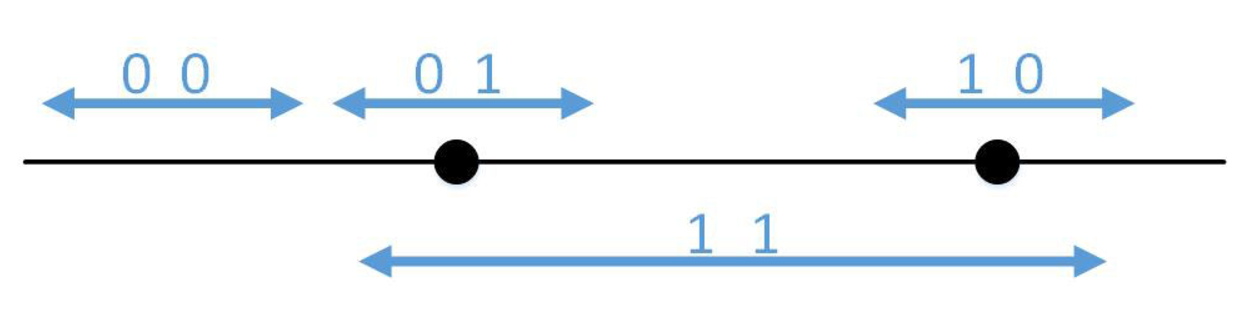
\includegraphics[width=2.1in]{notes1.eps}}
  \hspace{1in}
  \subfigure[]{
    \label{fig:subfig:b} %% label for second subfigure
    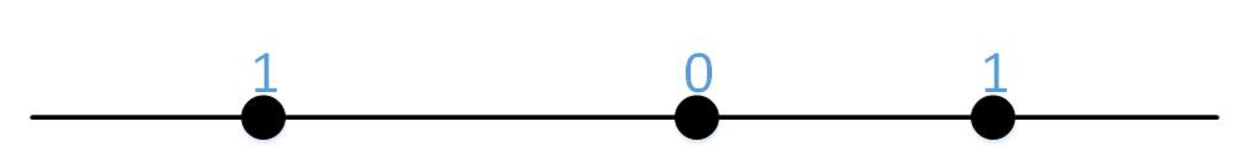
\includegraphics[width=2.1in]{notes2.eps}}
  \caption{VC dimension of intervals on the real line. (a) two points can always be shattered (b) three points cannot be shattered when it is $1, 0, 1$.}
  \label{fig:subfig} %% label for entire figure
\end{figure}
\end{tcolorbox}



\section{Covering Techniques}
Although Massart's lemma handles the finite hypothesis well, what if the set $Q$ is not finite? A simple solution would be making the set $Q$ finite by discretization, which reminds us of the covering technique covered in previous lecture. However, different from before, the randomness comes from $\{\sigma_i\}s$ instead of the data.\\\\
Recall the definition of a $\epsilon$-cover.
\begin{definition}[$\epsilon$-covering]
An $\epsilon$ cover of a set $Q$ is a set $C$ such that 
\[\forall x \in Q,\,\, \exists\, x' \in C,\,\,\, s.t.\,\,\, \rho(x, x') \leq \epsilon \qquad \text{where $\rho$ is some metric}\]
\end{definition}
What we want here is to discretize the space of the family of losses then apply Massart's lemma to bound the Rademacher Complexity of infinite hypothesis. In particular, notice that covering $Q$ w.r.t metric $||\cdot||_2$ is equivalent as covering the family of losses $\mathcal{F}$ w.r.t. $\rho = L_2(P_n)$, or more specically:
\[\rho(f, f') = \sqrt{\frac{1}{n}\sum_{i=1}^n\big(f(z_i) - f'(z_i)\big)^2}\qquad \text{for }f, f' \in \mathcal{F}\]
Finally, we introduce the following theorem that completes the connection from the Rademacher Complexity to the $\epsilon$ covering of $\mathcal{F}$.
\begin{theorem}
Let $\mathcal{F}$ be a family of functions from $z = (x, y) \longmapsto [-1,\,+1]$. Then
\[R_s(\mathcal{F}) \leq \inf\limits_{\epsilon} \underbrace{\sqrt{\frac{2\log N(\epsilon, \mathcal{F}, \rho)}{n}}}_{A} + \epsilon\]
\end{theorem}
Here $N(\epsilon, \mathcal{F}, \rho)$ denotes the minimum size of the $\epsilon$-cover of $\mathcal{F}$ w.r.t the metric $\rho$. Notice that there is a trade-off between $A$ and $\epsilon$, e.g. as $A$ goes up $\epsilon$ goes down and vice versa.
\begin{proof}
Let $C$ be the $\epsilon$-cover of $\mathcal{F}$ w.r.t $\rho$. In addition, let $B_\epsilon(g)$ denote the $\epsilon$ neighborhood of $g$ w.r.t $\rho$. Then
\begin{flalign*}
R_s(\mathcal{F}) &= \frac{1}{n}\E_{\sigma}\bigg[ \sup_{f \in \mathcal{F}}\sum_{i} \sigma_i f(z_i)\bigg] \\
&= \frac{1}{n} \E_\sigma \bigg[\sup_{g \in C} \sup_{f \in \mathcal{F} \cap B_\epsilon(g)} \sum_{i} \sigma_i f(z_i)\bigg] \qquad (\text{since } \mathcal{F} \subseteq \bigcup_{g\in C} B_\epsilon(g))\\
&= \frac{1}{n}\E_\sigma\bigg[\sup_{g\in C}\sup_{f \in \mathcal{F} \cap B_\epsilon(g)}\bigg( \sum_i \sigma_i \big(f(z_i) - g(z_i)\big) + \sum_i \sigma_i g(z_i)\bigg) \bigg]
\end{flalign*}
Notice that by Cauchy-Schwarz and the definition of $\epsilon$-cover,
\[
 \sum_i \sigma_i \big(f(z_i) - g(z_i)\big) \leq \sqrt{\bigg(\sum_i \sigma^2\bigg)\bigg(\sum_i \big(f(z_i)-g(z_i)\big)^2\bigg)} \leq n\epsilon\]
 Therefore
\begin{flalign*}
 R_s(\mathcal{F})&= \frac{1}{n}\E_\sigma\bigg[\sup_{g\in C}\sup_{f \in \mathcal{F} \cap B_\epsilon(g)}\bigg( \sum_i \sigma_i \big(f(z_i) - g(z_i)\big) + \sum_i \sigma_i g(z_i)\bigg) \bigg]\\
 &\leq 
 \frac{1}{n}\E_\sigma\bigg[\sup_{g\in C}\sup_{f \in \mathcal{F} \cap B_\epsilon(g)}\bigg( n\epsilon + \sum_i \sigma_i g(z_i)\bigg) \bigg] \\
 &= \frac{1}{n}\E_\sigma\bigg[\sup_{g\in C}\bigg( n\epsilon + \sum_i \sigma_i g(z_i)\bigg) \bigg] \qquad \text{(since there is no $f$ involved)}\\
 &= \epsilon + \frac{1}{n}\E_\sigma\bigg[\sup_{g\in C}\bigg(\sum_i \sigma_i g(z_i)\bigg) \bigg]\\
 &= \epsilon + R_s(C)
\end{flalign*}
Notice that we can pick whatever $\epsilon$ we want, combined with Massart's lemma, we have
\[ R_s(\mathcal{F}) \leq \inf_\epsilon \bigg(\epsilon + R_s(C)\bigg) \leq \inf\limits_{\epsilon} \sqrt{\frac{2\log N(\epsilon, \mathcal{F}, \rho)}{n}} + \epsilon \]
\end{proof}


%%%%%%%%%%%%%%%%%%%%%%%%%%%%%%%%%%%%%%%%%%%%%%%%%%%%%%%%%%%%%%%%
\bibliographystyle{plain}
\bibliography{10_22_final}
\end{document}
